\documentclass[tikz,border=5pt]{standalone}
\usepackage{pgfplots}\pgfplotsset{compat=1.18}
\definecolor{corba}{HTML}{3F51B5}\definecolor{guia}{HTML}{526CFE}\definecolor{punt}{HTML}{D32F2F}
\begin{document}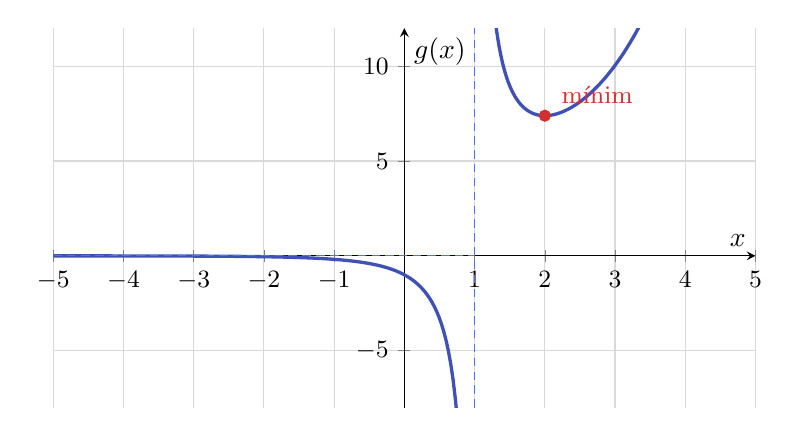
\begin{tikzpicture}
\begin{axis}[width=10.5cm,height=6.4cm,axis lines=middle,xmin=-5,xmax=5,ymin=-8,ymax=12,
 xlabel={$x$},ylabel={$g(x)$},grid=major,grid style={black!15},tick label style={font=\small},samples=180,clip=true]
 \addplot[corba,very thick,domain=-5:.96]{exp(x)/(x-1)};\addplot[corba,very thick,domain=1.04:5]{exp(x)/(x-1)};
 \addplot[guia,densely dashed] coordinates {(1,-8)(1,12)};\addplot[guia,densely dashed,domain=-5:1]{0};
 \addplot[only marks,mark=*,mark size=2pt,punt] coordinates {(2,7.389)};
 \node[anchor=south west,font=\small,text=punt] at (axis cs:2.1,7.5) {mínim};
\end{axis}\end{tikzpicture}\end{document}
